\documentclass[12pt, a4paper, oneside]{ctexart}
\usepackage{amsmath, amsthm, amssymb, appendix, bm, graphicx, hyperref, mathrsfs}
\usepackage{graphicx}

\title{\textbf{\textbf{关于PM2.5环境污染问题影响因素和预测模型研究}}}
\author{孔德睿\ 倪玉杰\ 马骁骏}
\date{\today}
\linespread{1.5}

%\newtheorem{theorem}{定理}[section]
%\newtheorem{definition}[theorem]{定义}
%\newtheorem{lemma}[theorem]{引理}
%\newtheorem{corollary}[theorem]{推论}
%\newtheorem{example}[theorem]{例}
%\newtheorem{proposition}[theorem]{命题}

\renewcommand{\abstractname}{\Large\textbf{摘要}}

\begin{document}

    %%%%%%%%%%%%%%%%%%%% Page 2 %%%%%%%%%%%%%%%%%%%%
    \thispagestyle{empty}
    \pagenumbering{Roman}
    \tableofcontents

    %%%%%%%%%%%%%%%%%%%% Page 1 %%%%%%%%%%%%%%%%%%%%
    \newpage
    \setcounter{page}{0}
    \maketitle
    \thispagestyle{empty}

    \begin{abstract}
        本文针对山东省若干市\textbf{PM2.5}指标变化及其与部分\textbf{气象因素}的相关性进行了研究。
        \par 首先,对来自PM2.5分析网及世界天气网部分数据进行收集整理。
        \par 针对问题(1),分别绘制PM2.5指标与气温、气压、风速、温度、降水量等部分气象因素散点图,通过计算\textbf{相关系数}对其时间的相关性进行分析,得到结论。
        \par 针对问题(2),首先,根据第(1)问的数据和相关性分析结果,利用部分年限的数据建立了PM2.5指标预测模型(\textbf{回归分析模型}),并通过线性回归方法得到系数。得出结论。
        其次,以\textbf{留出法}处理数据,通过计算模型\textbf{决定系数}以对其合理性做出评价,得到结论。
        \par 针对问题(3),首先,搜集并处理了北京市、上海市、(新疆)多年的PM2.5指标相关数据,绘制其随季节及年份变化散点图,分析其变化情况以及与山东省指标的差异,得到结论:
        并据此对山东省改善空气质量给出了合理化的政策建议。

        \par\textbf{关键词:} {PM2.5}\ {气象因素}\ {相关系数}\ {回归分析模型}\ {留出法}\ {决定系数}
    \end{abstract}


    %%%%%%%%%%%%%%%%%%%% Page 3 %%%%%%%%%%%%%%%%%%%%
    \newpage
    \setcounter{page}{1}
    \pagenumbering{arabic}

%    \section{一级标题}\label{sec:}
%    \subsection{二级标题}\label{subsec:}
%    \subsubsection{三级标题}\label{subsubsec:}
%    \paragraph{四级标题}\label{par:}
%    \subparagraph{五级标题}\label{subpar:}


    \section{问题重述与分析}
    问题重述:
    \par (1)针对山东省各市以往年份的PM2.5指标值,分析与其相关的各项影响因素,并进行相关性分析。
    \par (2)针对山东省各市以往年份的PM2.5指标以及影响因素,建立合理的预测模型,并对模型进行评价。
    \par (3)对照我国其他省份,分析山东省的PM2.5的变化情况与其他各省份PM2.5指标的差异与不同,给出合理化的政策建议。
    \par 问题分析:
    \par (1)需要找到各市以往年份的PM2.5指标值和与其可能有相关性的各指标数据,进行相关性分析,通过计算相关系数,判断相关性正负和相关程度。
    \par (2)首先,依照(1)的分析结果,需要对各指标的影响分别进行回归模型构建,再应用残差分析等方法进行模型评价和修正,加入时间因素,综合各种指标,构建完整预测模型。
    \par (3)需要收集其他各省(市)PM2.5指标值和与其可能有相关性的各种指标的数据,与山东省的指标进行比对,找到差异并分析不同的原因,再依此给出合理化的政策建议。


    \section{符号说明}

    $T$ :温度,单位 ${}^\circ C$
    \par $P$ :气压,单位:mmHg
    \par $U$ :相对湿度,单位: $\%$
    \par $Ff$ :风速,单位:m/s
    \par $RRR$ :降水量,单位:mm
    \par $CO$ :一氧化碳的浓度,单位:mg/m³
    \par $SO2$ :二氧化硫的浓度,单位:μg/m³
    \par $O3$ :臭氧的浓度,单位:μg/m³
    \par $PM2.5$ 或 $PM25$ :PM2.5的浓度,单位:μg/m³
    \par $t$ :时间,单位:月


    \section{模型假设}
    为了简化问题,作如下假设:
    \par (1)数据来源准确无误;
    \par (2)除本次研究的气象因素外,其他因素对PM2.5指标(以下简称指标)无显著影响。


    \section{指标分析及模型构建}

    \subsection{数据整理}
    把收集的数据整理成以“月”为单位的时间序列

    \subsection{问题(1)——判断指标与各气象因素的相关性}
    分别绘制济南(左)、青岛(中)、潍坊(右)三市指标与气象因素的散点图,如图[1][2][3]

    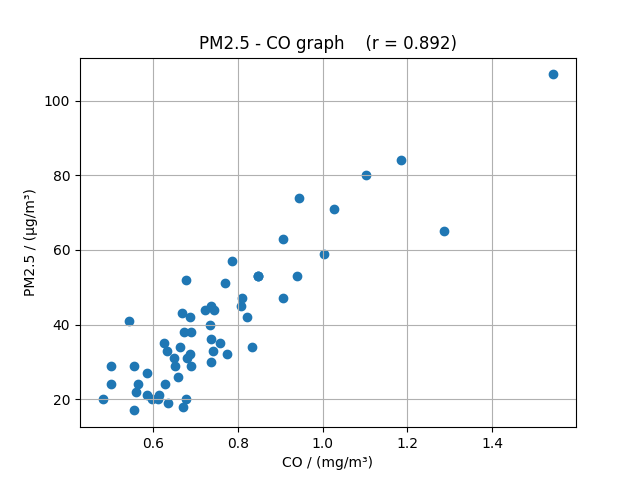
\includegraphics[width=0.33\linewidth]{./graph/CO/1}
    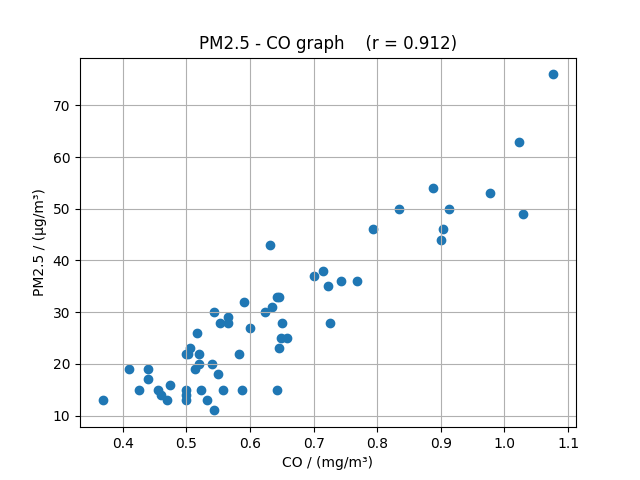
\includegraphics[width=0.33\linewidth]{./graph/CO/2}
    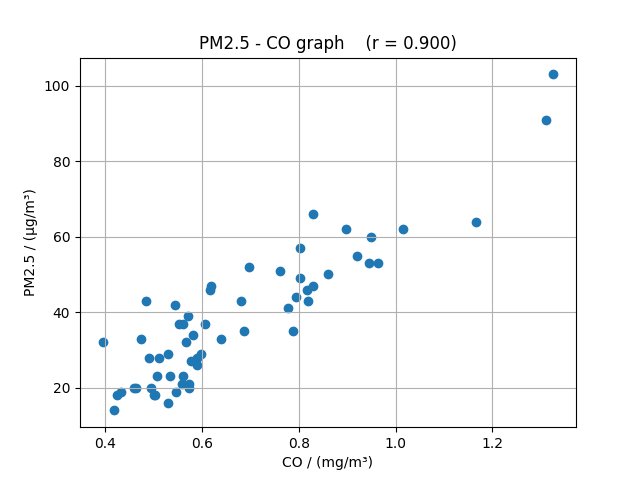
\includegraphics[width=0.33\linewidth]{./graph/CO/3}
    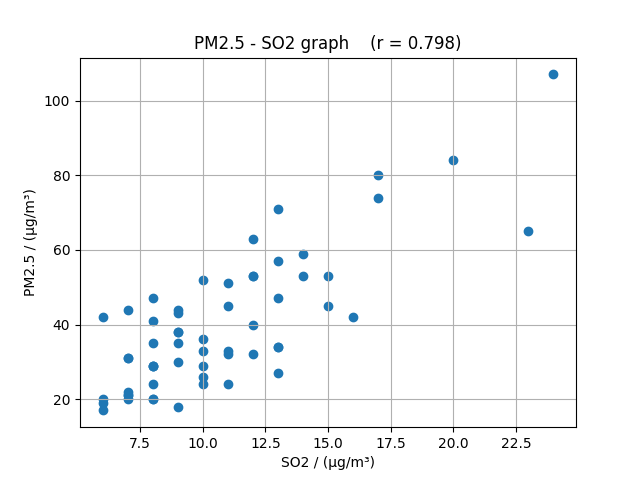
\includegraphics[width=0.33\linewidth]{./graph/SO2/1}
    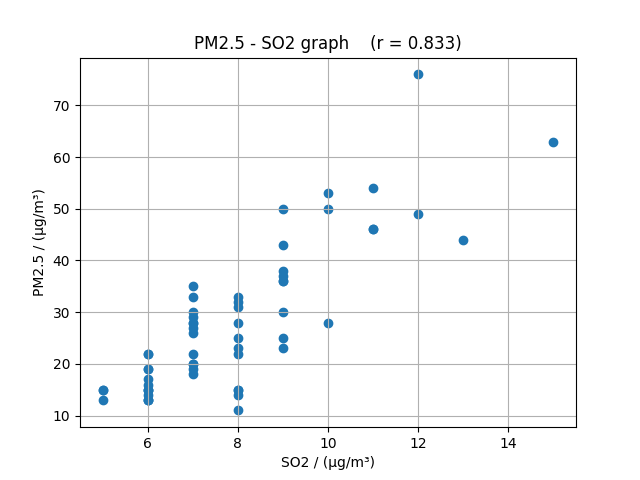
\includegraphics[width=0.33\linewidth]{./graph/SO2/2}
    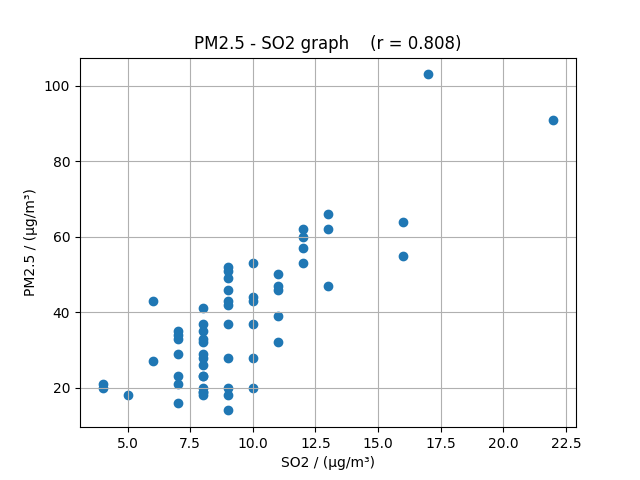
\includegraphics[width=0.33\linewidth]{./graph/SO2/3}
    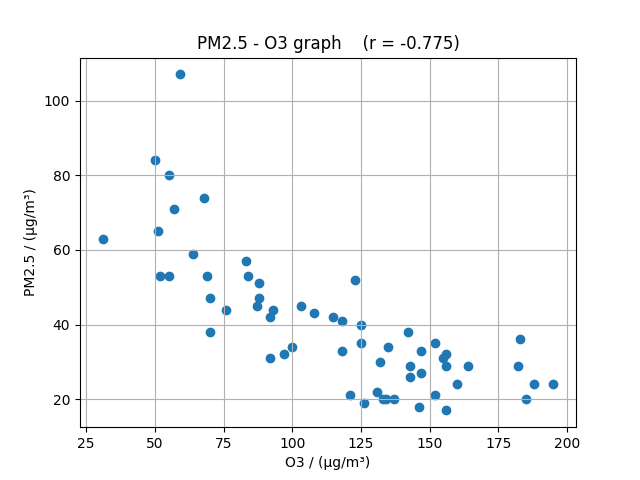
\includegraphics[width=0.33\linewidth]{./graph/O3/1}
    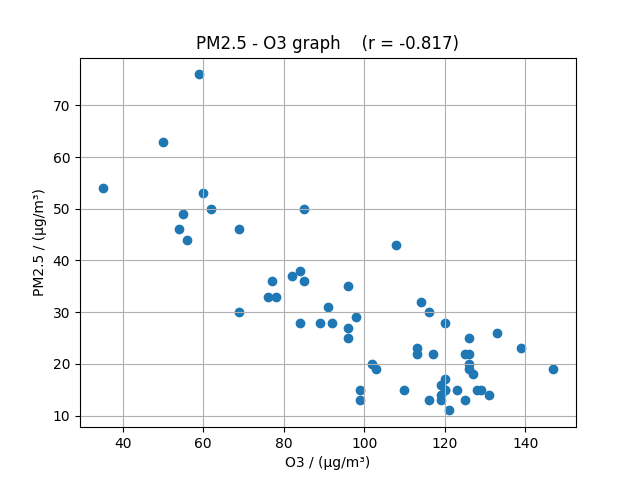
\includegraphics[width=0.33\linewidth]{./graph/O3/2}
    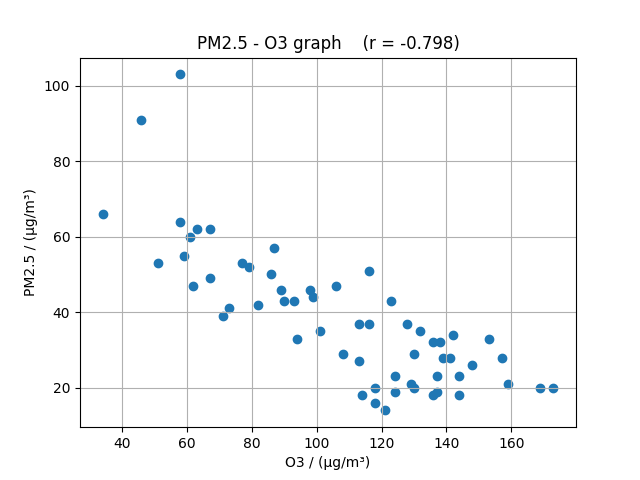
\includegraphics[width=0.33\linewidth]{./graph/O3/3}
    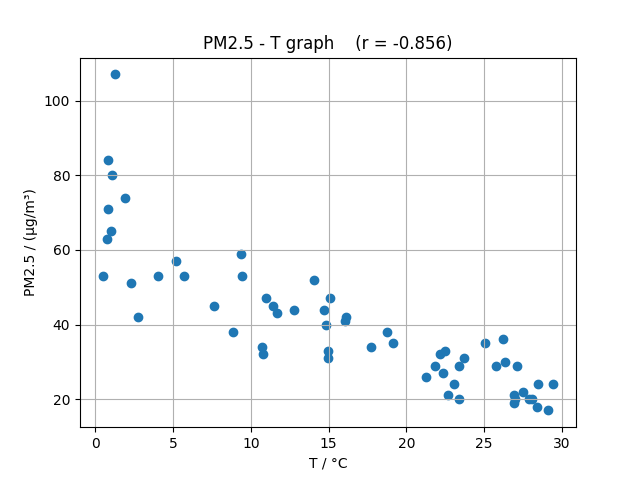
\includegraphics[width=0.33\linewidth]{./graph/T/1}
    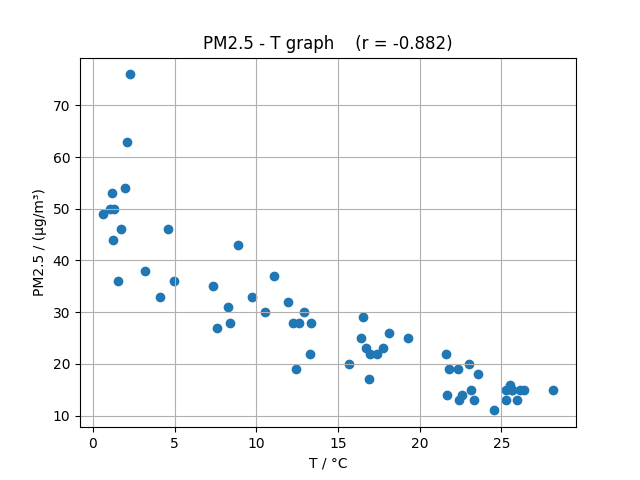
\includegraphics[width=0.33\linewidth]{./graph/T/2}
    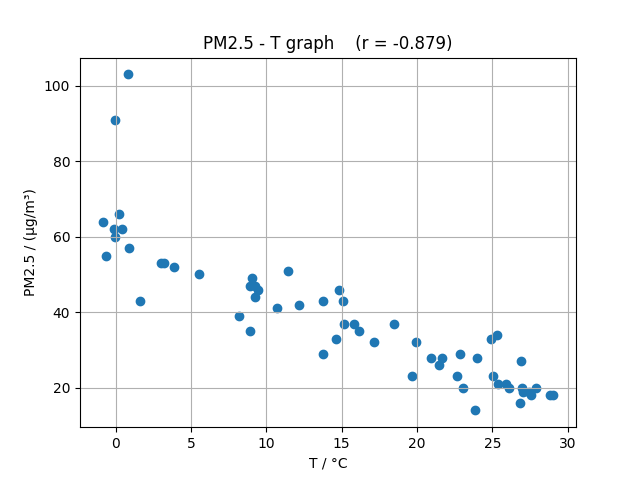
\includegraphics[width=0.33\linewidth]{./graph/T/3}
    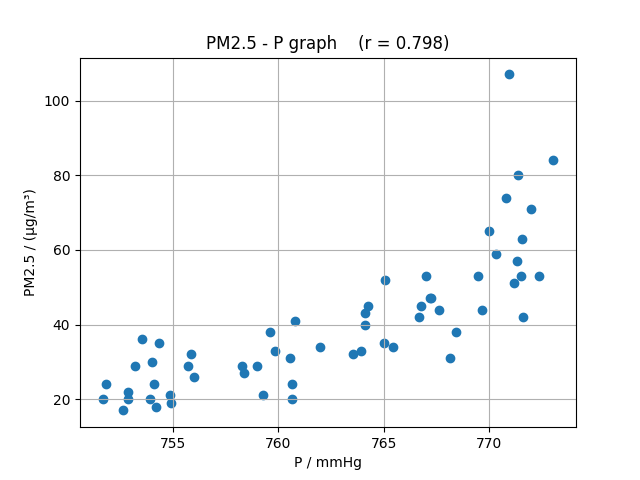
\includegraphics[width=0.33\linewidth]{./graph/P/1}
    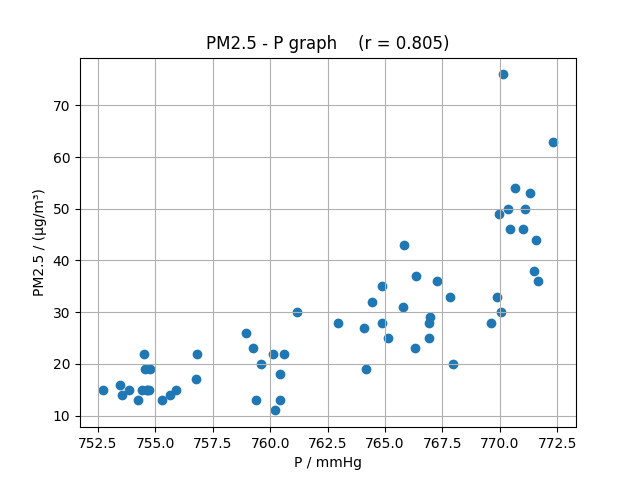
\includegraphics[width=0.33\linewidth]{./graph/P/2}
    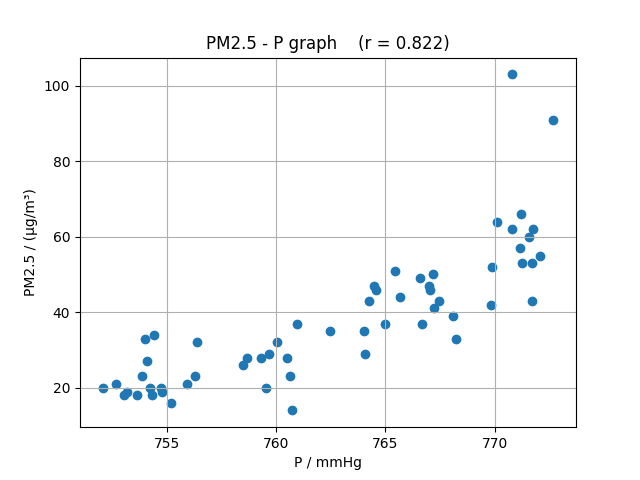
\includegraphics[width=0.33\linewidth]{./graph/P/3}
    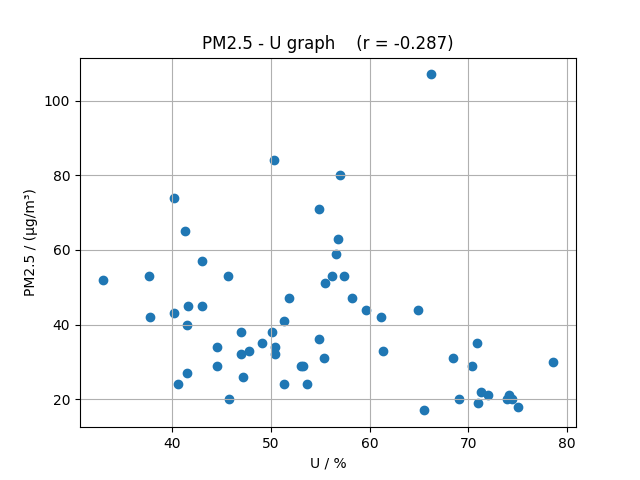
\includegraphics[width=0.33\linewidth]{./graph/U/1}
    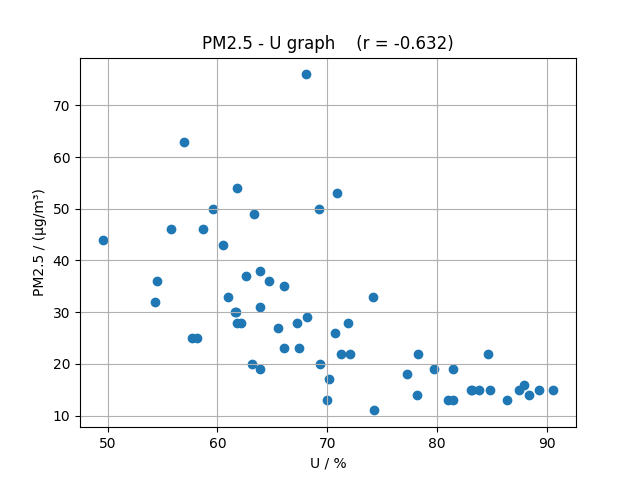
\includegraphics[width=0.33\linewidth]{./graph/U/2}
    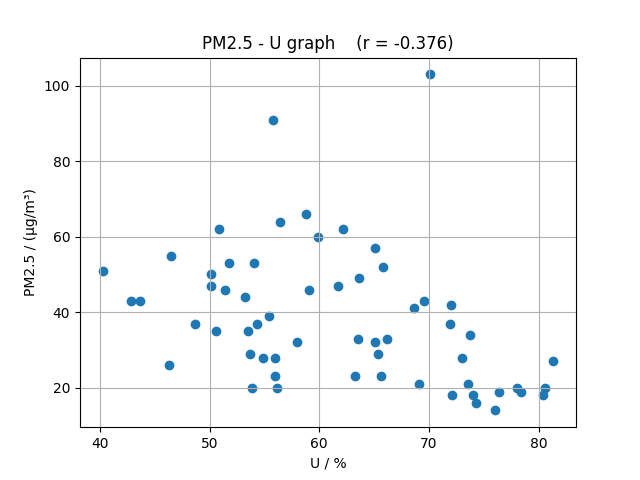
\includegraphics[width=0.33\linewidth]{./graph/U/3}
    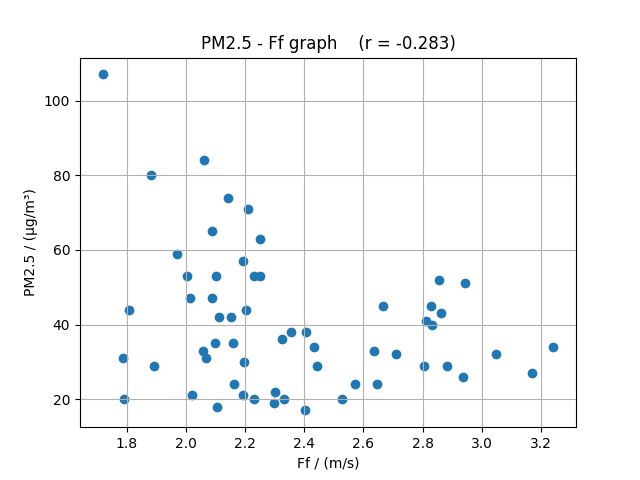
\includegraphics[width=0.33\linewidth]{./graph/Ff/1}
    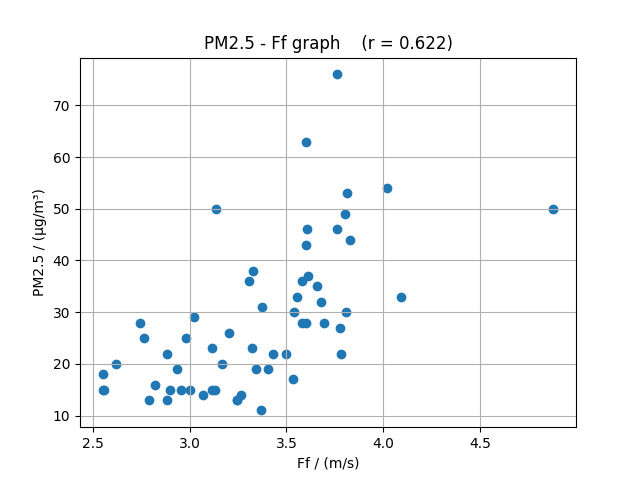
\includegraphics[width=0.33\linewidth]{./graph/Ff/2}
    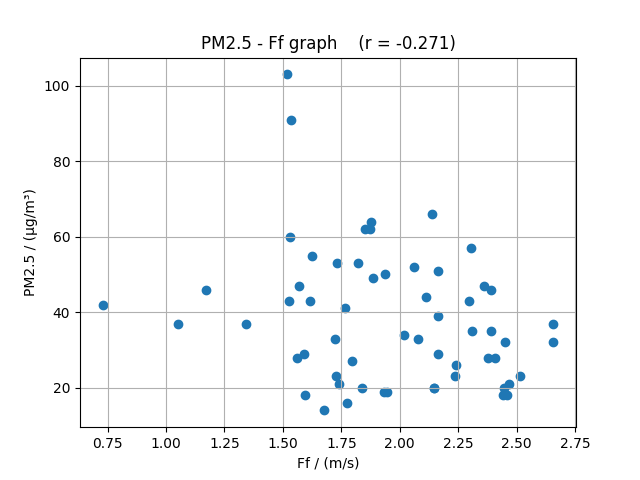
\includegraphics[width=0.33\linewidth]{./graph/Ff/3}
    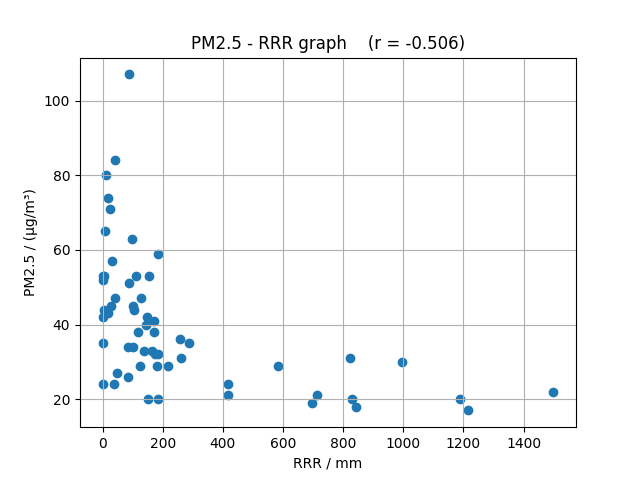
\includegraphics[width=0.33\linewidth]{./graph/RRR/1}
    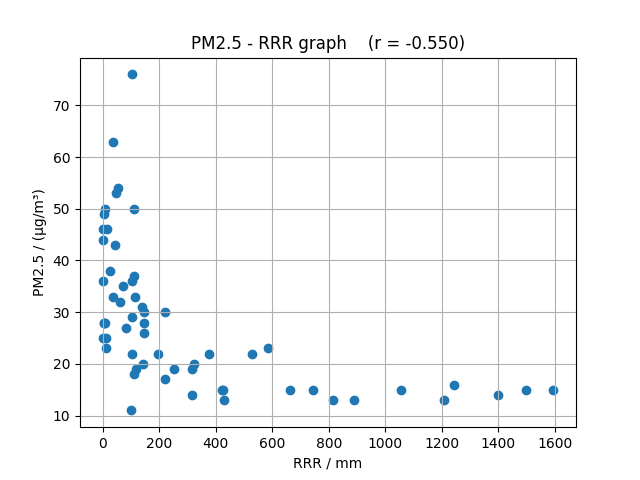
\includegraphics[width=0.33\linewidth]{./graph/RRR/2}
    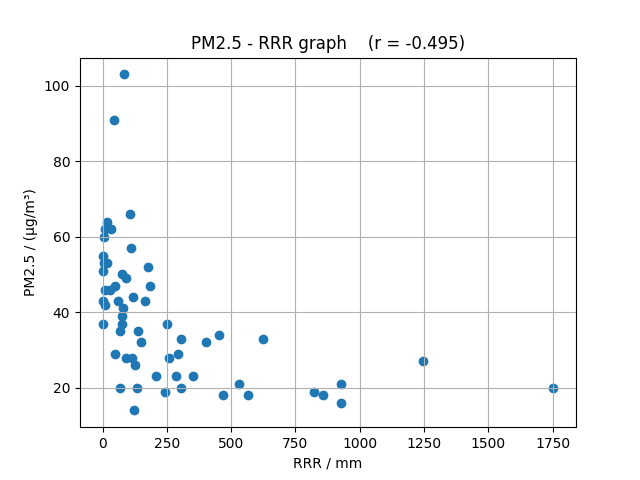
\includegraphics[width=0.33\linewidth]{./graph/RRR/3}

    由图可得,指标与P、CO呈线性正相关,与T、O3呈线性负相关,与RRR呈负相关但不显著,与Ff、U无显著关系。

    \subsection{问题(2)——建立指标的预测模型}

    \subsubsection{建立指标与气象因素综合的回归模型}
    绘制济南、青岛、潍坊三市指标随时间变化折线图[2]

    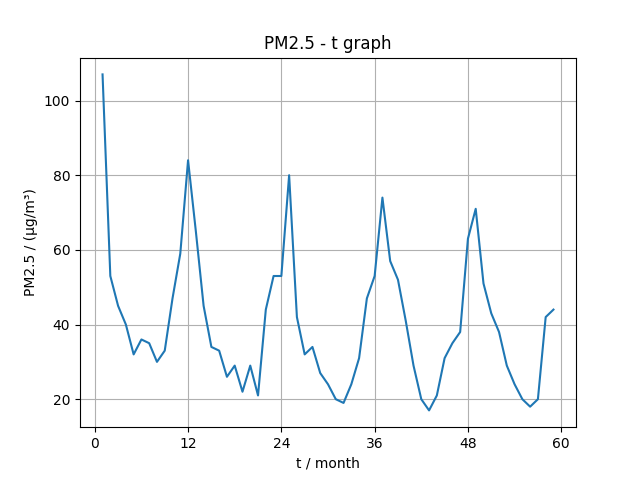
\includegraphics[width=0.33\linewidth]{graph/PM25t/1}
    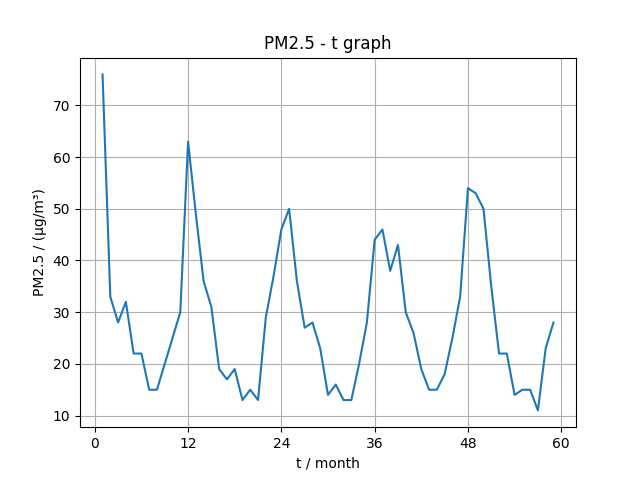
\includegraphics[width=0.33\linewidth]{graph/PM25t/2}
    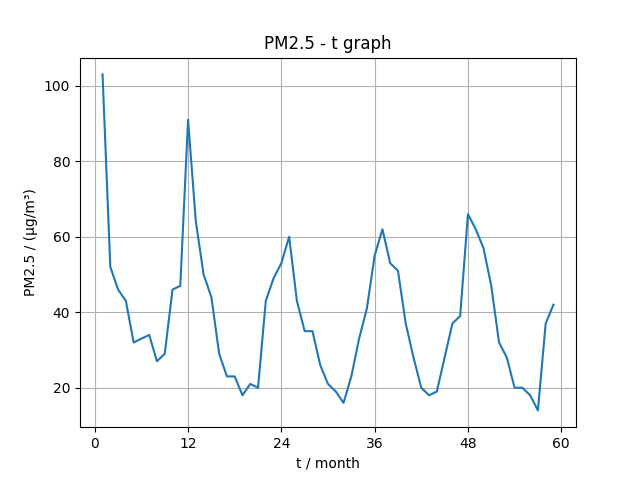
\includegraphics[width=0.33\linewidth]{graph/PM25t/3}

    发现其一年内具有明显的周期性,以年为尺度具有线性负相关性。结合4.2分析结论,以此构建 PM25 对各气象因素综合的回归模型:
    \[PM25=\beta_1 \cdot CO + \beta_2 \cdot O3 + \beta_3 \cdot T + \beta_4 \cdot P + \beta_5 \cdot t + \beta_6 \cdot \sin\dfrac{6}{\pi}t + \epsilon\]
    对2013年12月到2024年11月数据进行最小二乘法拟合得(详见附件代码)[4]:
    \[PM25=55.8695\ CO + 0.1105\ O3 -1.1326\ T + 0.0210\ P -0.1609\ t -0.6618\ \sin\dfrac{6}{\pi}t + 4.3032\]

    \subsubsection{模型评价}
    应用留出法评价,将2013年12月到2023年12月数据作为训练集,将2024年各项因素的数据作为测试集,带入预测模型,得到每个月的指标预测值,绘制折线图,与实际值比较,如图

    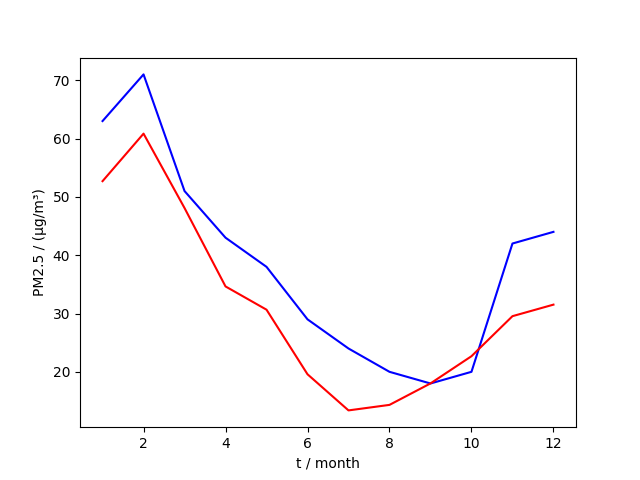
\includegraphics[width=\linewidth]{./graph/predict}

    决定系数 $R^2 = 0.992$
    \par 从图中可知,预测值十分接近实际值,$R^2>0.99$ 可知该模型拟合效果极好。

    \subsection{问题(3)——分析山东省与其他省指标变化的不同并给出政策建议}
    绘制出北京市(左上)、上海市(右上)、重庆市(左下)和山东省(以济南为例)(右下)指标的折线图,如图

    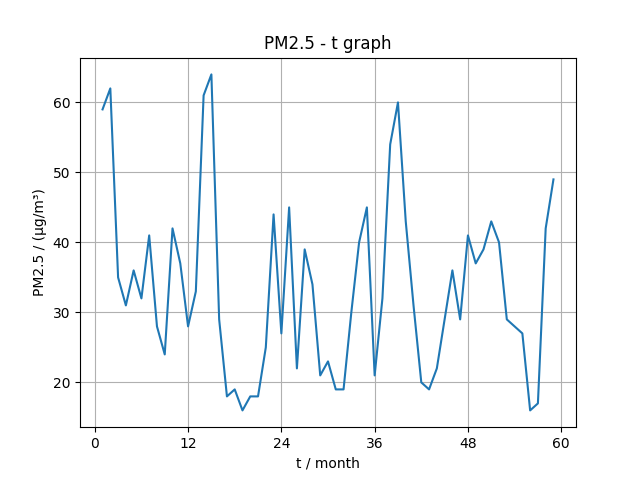
\includegraphics[width=0.5\linewidth]{./graph/PM25t/b}
    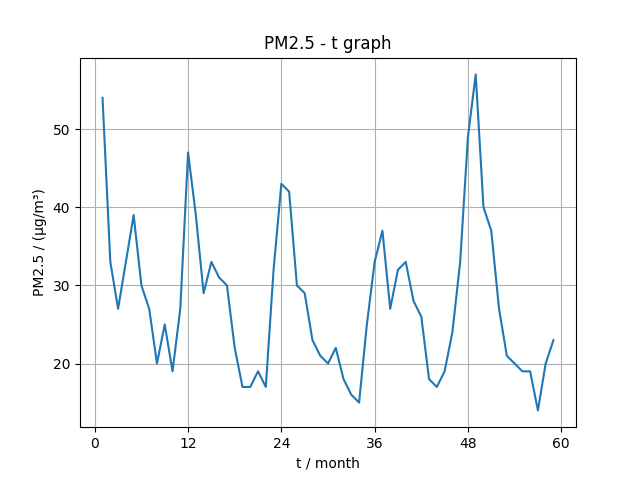
\includegraphics[width=0.5\linewidth]{./graph/PM25t/s}
    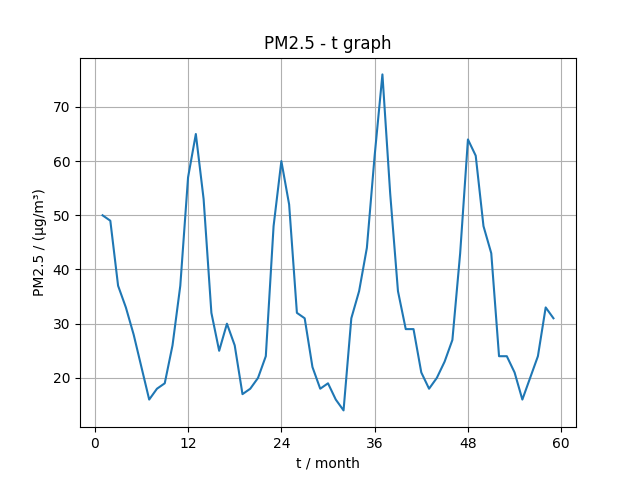
\includegraphics[width=0.5\linewidth]{./graph/PM25t/c}
    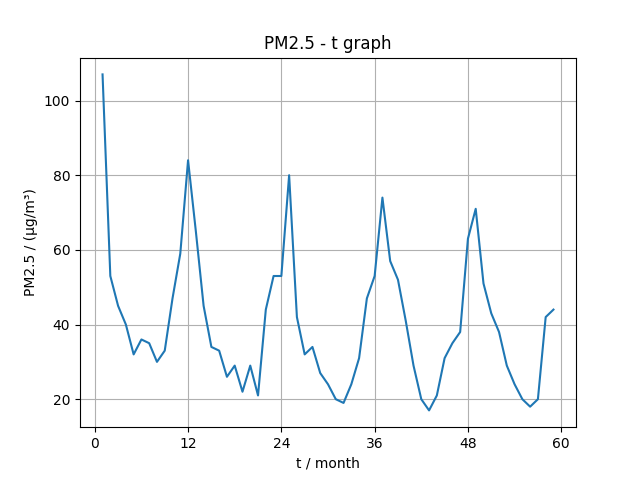
\includegraphics[width=0.5\linewidth]{./graph/PM25t/1}

    发现山东省指标普遍偏高,但随年份呈下降趋势。
    \par 查阅资料[5]得,山东省重工业发达,但高新产业增势强劲。
    \par 依据上述分析,可以给出如下政策建议:
    \par 1. 促进工业废气排放多,环境污染影响大的重工业传统企业转型升级。
    \par 2. 推动高新产业发展,转换增长动能,在降低PM2.5等环境污染同时保证经济发展稳中向好。


    \section{模型的反思与推广}

    \subsection{模型优点}
    (1)分析各气象因素对指标影响时,运用相关系数 $r$ 分析其相关性。
    \par (2)在建立指标的预测模型时,运用了线性回归模型,通过合理分析修正模型,提高模型准确度,并用留出法对模型进行检验。
    \par (3)分析山东省指标变化与其他各省份指标的差异时,从季节(月份)、年份多角度进行比较。

    \subsection{模型缺点}
    (1)对于不同城市由于不同地理位置造成的气候差异未进行分析。
    \par (2)考虑因素之间相关性较强,但实际上各因素之间并非完全独立,存在共同影响。

    \subsection{模型推广}
    本文所得出的模型或方法可以推广到其他有关气象数据的研究中,在实践中对PM2.5指标的准确预测有促进作用。

    %%%%%%%%%%%%%%%%%%%% Page 4 %%%%%%%%%%%%%%%%%%%%
    \newpage

    \begin{thebibliography}{9}
        \bibitem{a} 世界天气网(https://rp5.ru)
        \bibitem{b} PM2.5分析网(https://www.aqistudy.cn)
        \bibitem{c}人教版A版 高中数学选修三 P98
        \bibitem{d}人教版A版 高中数学选修三 P105-120
        \bibitem{e}朱玲珍.山东工业高质量发展呈五大特点.电子信息产业网(www.cena.com.cn)
    \end{thebibliography}

    %%%%%%%%%%%%%%%%%%%% Page 5 %%%%%%%%%%%%%%%%%%%%
    \newpage

    \begin{appendices}
        \renewcommand{\thesection}{\Alph{section}}


        \section{附录}\label{sec:2}
        \par 问题(1) 程序(python)(ploting\_PM25\_weather\_air.py)
        \par 问题(2) 程序及结果(python)(ploting\_PM25\_time.py、linear\_regression.py、linear\_regression\_predict.py)
        \par 问题(3) 程序(python)(ploting\_PM25\_time.py)
    \end{appendices}

\end{document}
